\documentclass{acmconf}
\usepackage{amssymb}
\usepackage{amsmath}
\usepackage{amstext}
\usepackage{proof}
\usepackage{code}
\usepackage{epsfig}
\usepackage{graphics}
\usepackage{psfrag}
\usepackage{color}
\usepackage{pstricks,pst-node,pst-tree}

\newcommand{\mygray}{\color{green}}
\newcommand{\mygreen}{\color{green}}

\newcommand{\bangforbindingcolon}{\mathcode`!="003A}
\bangforbindingcolon
\def\sig{\mathsf{sig}}
\def\ctx{\mathsf{ctx}}
\def\kind{\mathsf{kind}}
\def\typeb{\mathsf{type}}
\newcommand{\figfoot}{\vspace{1ex}\hrule}
\newcommand{\fighead}{\hrule\vspace{1.5ex}}

\newcommand{\z}{\mbox{}}

%\newcommand{\typeLF}{\textsf{type}}
%\newcommand{\propLF}{\textsf{prop}}

%\newcommand{\false}{\textsf{false}}
%\newcommand{\true}{\textsf{true}}
%\newcommand{\andLF}{\; \textsf{and}\;}
%\newcommand{\impLF}{\;\textsf{imp}\;}
%\newcommand{\forallLF}{\;\textsf{forall}\;}
%\newcommand{\existsLF}{\;\textsf{exists}\;}
%\newcommand{\eqLF}{\;\textsf{eq}\;}
%\newcommand{\eqilLF}{\;\textsf{eqi1}\;}
%\newcommand{\eqirLF}{\;\textsf{eqi2}\;}
%\newcommand{\eqalLF}{\;\textsf{eqa1}\;}
%\newcommand{\eqarLF}{\;\textsf{eqa2}\;}

% spine notation
% \newcommand{\nil}{\textsc{nil}}
\newcommand{\comb}{\cdot}


\newcommand{\pfLF}{\tt{prov}}
\newcommand{\typeLF}{\tt{type}}
\newcommand{\propLF}{\tt{prop}}

\newcommand{\false}{\tt{false}}
\newcommand{\true}{\tt{true}}
\newcommand{\andLF}{\tt{and}\;}
\newcommand{\impLF}{\tt{imp}\;}
\newcommand{\forallLF}{\tt{forall}\;}
\newcommand{\existsLF}{\tt{exists}\;}
\newcommand{\eqLF}{\tt{eq}\;}
\newcommand{\eqilLF}{\tt{e1}}
\newcommand{\eqirLF}{\tt{e2}}
\newcommand{\eqalLF}{\tt{e3}}
\newcommand{\eqarLF}{\tt{e4}}

\newcommand{\orl}{\vee}
\newcommand{\andl}{\wedge}
\newcommand{\impl}{\supset}
\newcommand{\ldot}{.\,}
\newcommand{\unif}{\;\doteq\;}

%\newcommand{\andI}{\textsf{andI}}
%\newcommand{\andEL}{\textsf{andE}$_1$}
%\newcommand{\andER}{\textsf{andE}$_2$}
\newcommand{\impI}{\textsf{impI}}
\newcommand{\allI}{\textsf{allI}}
\newcommand{\allE}{\textsf{allE}}
%\newcommand{\orIR}{\textsf{orI}$_1$}
%\newcommand{\orIL}{\textsf{orI}$_2$}
%\newcommand{\orE}{\textsf{orE}}
%\newcommand{\exI}{\textsf{exI}}
%\newcommand{\exE}{\textsf{exE}}
\newcommand{\impE}{\textsf{impE}}
\newcommand{\ax}{\textsf{axiom}}
%\newcommand{\trueI}{\textsf{trueI}}
%\newcommand{\falseE}{\textsf{falseE}}

\newcommand{\listd}{\mathsf{list }}
\newcommand{\chars}{\mathsf{char}\;}
\newcommand{\integer}{\mathsf{int}\;}
\newcommand{\nil}{\mathsf{nil}}
\newcommand{\conc}{\;;\;}
\newcommand{\cons}{\mathsf{cons }\;}

\newcommand{\vd}{\vdash}
\newcommand{\vdN}{\Vdash}
\newcommand{\arrow}{\rightarrow}
\newcommand{\hastype}{\mathrel{:}}
\newcommand{\oftp}{\mathord{:}}
\newcommand{\ofvd}{\mathord{::}}
\newcommand{\lam}{\lambda}
\newcommand{\turn}{\mathord{\scriptstyle \vdash}}

\newcommand{\ednote}[1]{\footnote{\it #1}}
\newenvironment{note}{\begin{quote}\message{note!}\it}{\end{quote}}

\newcommand{\lbb}{{[\![}}
\newcommand{\rbb}{{]\!]}}
\newcommand{\Mu}{\lbb M/u\rbb}
\newcommand{\id}{\mathsf{id}}
\newcommand{\msub}[1]{\lbb #1 \rbb}
\newcommand{\inv}[1]{{#1}^{-1}\,}

\newcommand{\type}{\mathsf{type}}
\newcommand{\mctx}{\;\mathsf{mctx}}

\newcommand{\bnfas}{\mathrel{::=}}
\newcommand{\bnfalt}{\mathrel{|}}

\begin{document}
\title{Generating and checking small proof witness for the logical
  framework LF}
\author{
\hspace{1cm}Susmit Sarkar
\hspace{2.5cm}
Brigitte Pientka\thanks{This work has been partially supported by NSER
  Grant ??? and FQRNT Grant ???}
\\ Carnegie Mellon University \hspace{1cm} McGill University
\\Pittsburgh, PA, USA \hspace{2cm}Montreal, CA
}

\affiliation{}
\maketitle 

\abstract{Certified code systems demand the production of small-sized
objects which can witness proofs in a machine-verifiable manner. We
present a proof compression and verification engine for the logical
framework LF. This extends ideas previous work by Necula and
Rahul~\cite{Necula+01:oracle} in two main ways: 1) We consider the full
fragment of LF 2) We will incorporate caching of sub-proofs to
generate even more compact proof representations. This demonstrates
that many of the restrictions 

Our system is integrated into the Twelf system, which has been widely
used for certified code systems, and a wide range of experimental
results demonstrates the practicality and usefulness of proof
compression within logical frameworks.}

\section{Introduction}
Proof-carrying code applications establish trust by verifying
compliance of the code with a given safety and security policy.
A code producer verifies that the program is safe to
run according to some predetermined safety policy, and supplies a
binary executable together with its safety proof. Before
executing the program, the code consumer then quickly checks the code's
safety proof against the binary. 

Many proof-carrying code projects, in particular in foundational PCC,
have employed the logical framework LF as a general safety
infrastructure for encoding safety polices and representing safety
proofs\cite{AppelFelty00,Crary:POPL03,AppelFelten99,Crary:CADE03}.
The main advantage of using a logical framework is its flexibility
and its small trusted computing base. Hence, it reduces the effort
required for each particular safety policy. However, proofs within the
logical framework may be large in size 
% several mega-bytes - with LFi few tens of kilobytes (=two orders of
% magnitude) 
, e.g. 4-times as big as the actual machine code. This has spawned a
number of research contributions to reduce proof size and proof
checking time for proof-carrying code applications. However, all these
contributions 
trade the expressive power and complexity of LF against
simplicity. 
In a first step, Necula and Lee's \cite{Necula98lics} developed a
proof representation for LF$_i$, essentially a restriction to 2-level
logical framework, which eliminated many implicit type information in
the representation of proofs. However, proofs in LF$_i$ are still
4-times as big as the program they are certifying.
To obtain even smaller proofs (1/8th the size of the machine code),
Necula proposed in \cite{Necula+01:oracle} to only record the
non-deterministic choices which were made when constructing the proof,
and then use a guided first-order logic programming engine to
reconstruct the proof on the consumer side. This simple idea leads to
small proof witnesses, sometimes called oracles, and has been
proven to be effective in many practical examples, and most recently
has been proposed within the Open Verifier Framework \cite{Necula?}. Wu
{\em{et. al}} \cite{Appel:PPDP03} use a similar idea for creating a
foundational proof checker with small witnesses. However, all these
approaches are restricted to simply typed Prolog-like engines which
work on the fragment of hereditary Harrop formulas. Although theses
approaches allow dynamic assumptions, they disallow a a higher-order
term language where terms can be defined using
$\lambda$-abstraction. This means they can only support first-order
abstract syntax rather than higher-order abstract syntax.  The main
reason for staying with a simple first-order term language are that
unification is decidable and easily implemented. Moreover, term
indexing techniques are well-known and well-understood for first-order
terms, hence allowing a straightforward implementation of Prolog-like
engines to compress and reconstruct proofs. 

%two-folded: First, in simple safety policies about typed-assembly
%language, higher-order abstract syntax is rarely used. However, as we
%move to more complex safety policies, support for higher-order
%abstract syntax will become more desirable. Second, techniques needed
%to extend oracle-based proof compression and proof re-construction for
% higher-order terms have been 

However, the lack of support for higher-order abstract syntax
encodings, means that any variable binding constructs must be
explicitly encoded. For example, Wu {\em et al}\cite{Appel:PPDP03}
encode the explicit substitution calculus \cite{Abadi:POPL90} together
with the necessary proofs about substitutions for their foundational
implementation of LTAL. The overhead in their setting is still
manageable although annoying, since simple safety policies about
typed assembly require variable binding constructs only in few
places. However, as we move beyond proving memory safety, we predict
that richer safety policies and type systems will play a more
important role in proof-carrying code applications. For these richer
language, support for higher-order abstract syntax will be
crucial. 

However, small proof
witnesses not only play a role in certifying code, but are useful and
sometimes necessary in building in certifying theorem proving and
logic programming engines. First, constructing and possibly storing
full proof terms is expensive, considering the fact that the size of
the proof term can be at least 4-times as big as the statement we are
trying to prove. Hence witnesses provide a cheap
simple alternative. As an example consider tabled higher-order logic
programming, where we memoize subgoals together with their answers and
proofs to re-use the results later. Constructing and storing the full
proof term however would impose a substantial performance
penalty. Hence, small witnesses provide a cheap
simple alternative and are in fact crucial to obtain a practical
tabled logic programming interpreter. Second, there has been interest
in producing proof justifiers in the logic programming community to
ease debugging. Small proof witnesses can be viewed as proof
justifiers and may be used to re-trace the proof. 

In this paper, we describe the design of the generation and checking
of small proof witnesses for full LF. This demonstrates that many of
the existing restrictions which are placed on existing oracle-based proof checkers
are unnecessary. The main obstacle in building a oracle-based proof checker for full LF
is due to higher-order terms (e.g. terms my contain
$\lambda$-abstraction). As a consequence, known oracle-based proof checking
systems entirely avoid this problem and concentrate in
practice on the first-order 
fragment, where for example unification is decidable and easily
implemented and efficient term indexing operations are known to make
it practical\footnote{Necula describes some higher-order extensions,
  ...}. In this paper, we demonstrate it is possible to extend
Twelf with making it unnecessary to build separate proof checking
engines. 
We propose the use of higher-order substitution tree indexing together
with linear higher-order pattern unification to extend oracle-based
proof checking to the higher-order setting. Furthermore, we improve on
the size of oracle-proofs by factoring out common
sub-proofs\footnote{Eliminating common sub-proofs is an orthogonal
  problem to eliminating redundant implicit type 
  information, as is   proposed in \cite{Necula98lics}.} by
incorporating memorization techniques. Identifying and factoring out
common sub-proofs leads to more compact oracles and can  
decrease proof-checking time by a factor of ?? since common sub-proofs
are only checked once.  We hope this will provide a comprehensive
guide for future implementations of proof checkers which need not be
restricted to first-order Prolog-like systems. In particular, various
certified code systems can exploit this idea. We have implemented 
a oracle-based proof generator and checker as part of the logical
framework {\em Twelf}.  

The paper is structured as follows. We give background on
higher-order logic programming in Twelf in Section~\ref{sec:twelf}. In
Section~\ref{sec:oracles}, we present our approach to oracle-based
proof generation and proof checking. In particular, we explain
higher-order term indexing to index higher-order logic programming
clauses. In Section~\ref{sec:tabling}, we discuss memoization techniques for
factoring out common subproofs. We conclude with a discussion of some
experimental results within Twelf and discussion of related work.

\section{Higher-order logic programming}\label{sec:twelf}

Higher-order logic programming extends first-order logic programming
in three main ways: First, first-order terms are replaced with
(dependently) typed $\lambda$-terms. Second, the body of clauses may
contain implications and universal quantification, thereby generating
dynamic assumptions which may be used during proof search. Thirdly,
execution of a query will not only produce a yes or no answer, but
generates a proof term as a certificate which can be checked
independently. These features make higher-order logic programming an
ideal generic framework for implementing formal safety policies given via
axioms and inference rules and executing them.

The theoretical foundation underlying higher-order logic programming
within Twelf is the LF type theory, a dependently typed lambda
calculus. In this setting types are interpreted as clauses and goals and
typing context represents the store of program clauses available. We
will use types and formulas interchangeably. Types and programs are
defined as follows: 

\begin{center}
\begin{tabular}[h]{lcl}
Types  $A$ & ::= & $P \mid  A_1 \rightarrow A_2 \mid \Pi x:A_1.A_2$ \\
Programs  $\Gamma$ & ::= & $\cdot \mid \Gamma, x:A$ 
\end{tabular}
\end{center}

$P$ ranges over atomic formulas and we interpreter the function arrow
$A_1 \rightarrow A_2$ as implication. The $\Pi$-quantifier, denoting
dependent function type, corresponds to the  universal
$\forall$-quantifier. Every type has a corresponding proof term $M$
and we assume that all proof terms are in normal form. To represent
proof terms, we use the spine notation~\cite{CervesatoPfenning01}. 

\begin{center}
\begin{tabular}[h]{lcl}
Terms  $M$ & ::= & $c \comb S \mid x \comb S \mid \lambda x. M $  \\ 
Spines $S$ & ::= & $\nil \mid M;S\;$
\end{tabular}
\end{center}

Other higher-order logic programming languages of a similar
flavor are $\lambda$-Prolog \cite{Nadathur99cade} or
Isabelle\cite{Paulson86}. To illustrate the notation and explain the
problem of small proof witnesses, we will first give an example of
encoding the natural deduction calculus in the logical framework LF
using higher-order logic programming following the methodology in
\cite{Harper93jacm}. For more information on how to encode formal
systems in LF see \cite{Pfenning97}.  Using this example, we will
explain oracle-based proof generation and proof-checking.  

\subsection{Representing Logics}
As a running example, we will consider intuitionistic logic formulated
in the natural deduction style. We will only concentrate on the fragment
consisting of implications and universal quantifiers. Propositions can
be then described as follows
\[
\begin{array}{llll}
\mbox{Propositions} & A,B, C & := & \top \mid A \impl B \mid \forall x.A \\
\mbox{Context} & \Gamma & := & \ldot \mid \Gamma,  A
\end{array}
\]

Inference rules describing natural deduction are presented in Table~\ref{natded}.

\begin{table}[h]
\fighead
\[
\infer{\Gamma\vdash \forall x. A}
{\Gamma\vdash [a/x]A & a \mbox{ is new}}
\qquad
\infer{\Gamma\vdash [T/x]A}
{\Gamma\vdash \forall x.A}
\qquad
\infer{\Gamma, A \vdash A}
{}
\]
\[
\infer{\Gamma\vdash A\impl B}
{\Gamma,A\vdash B}
\qquad
\infer{\Gamma\vdash B}
{\Gamma\vdash A\impl B
\quad
\Gamma\vdash A}
\]
\figfoot
\caption{\label{natded}A natural deduction system}
\end{table}

To represent this system in LF, we first need formation rules to
construct terms for the objects we are talking about, in this case,
propositions. We declare a new type {\tt prop} for propositions and a
type {\tt i} for individuals. We intend that terms belonging to {\tt
  prop} represent well-formed propositions. The rules are given below,
in concrete Twelf syntax. Throughout the example we reverse the arrow {\tt{A -> B}} writing instead {\tt{B <- A}}. From a logic programming view, it might be more intuitive to think of the clause {\tt{H <- A$_1$ <- A$_2$ <- $\ldots$ <- A$_n$}} as {\tt{H <- A$_1$, A$_2$, $\ldots$, A$_n$}}.

%prop : type.
%i    : type.
%\vspace{0.1in}
%false  : prop.
%true   : prop.

\begin{code}
imp    : prop -> prop -> prop.
forall : (i -> prop) -> prop.
\end{code}

The connectives for implication takes in two propositions and returns a
proposition. To represent the forall-quantifier, we will use
higher-order abstract syntax. The crucial idea is to represent bound
variables in the object language (logic) with bound variables in the
meta-language (higher-order logic programming). 

Next we turn our attention to the proofs in our system. We have a
judgment for provability within this logic, which we denote by the
type family {\tt prov}.
%
%\begin{code}
% prov : prop -> type.
%\end{code}%
%
Each clause will correspond to an inference rule in the object
logic. For convenience, we give the constructors 
descriptive names, and follow the order of the rules in
Table~\ref{natded}. 

\begin{code}
alli   : prov (forall $\lambda$x. A x)
            <- $\Pi$x. prov (A x)
alle   : prov (A T)
            <- prov (forall $\lambda$x. A x).
\z
impi     : prov (imp A B)
            <- (prov A -> prov B).
impe     : prov B
            <- prov (imp A B)
            <- prov A.
\end{code}

%\z
%truei    : prov true.
%\z
%falsee   : prov C
%            <- prov false.

These rules are given as a Twelf signature. $A$, $B$, $C$ denote
existential or logic variables which are instantiated during proof
search. There are two key ideas which make the encoding of the sequent
calculus elegant and direct. First, we use the power of dynamic
assumptions which higher-order logic programming provides, to
eliminate the need to manage assumptions in a list explicitly. To
illustrate, we consider the clause {\tt impI}. To  prove {\tt prov
  (imp A B)}, we prove {\tt prov B} assuming {\tt prov A} In other words,
the proof for {\tt prov B} may use the dynamic assumption {\tt prov A}. 

Second, we use higher-order abstract syntax to encode the bound
variables in the universal quantifier. As a consequence substitution
in the object language can be reduced to application and
$\beta$-reduction in the meta-language (higher-order logic
programming). Consider the rule for all-elimination. If we have a proof of
$\forall x.A$ , then we know that $[T/x]A$ is true for any term
$T$. The substitution $[T/x]A$ in the object language is achieved via
application in the meta-language {\tt (A T)}. 



\subsection{Proof search in higher-order logic programming}

Higher-order logic programming is similar to a Prolog interpreter
since it performs essentially a depth-first search over all the
program clauses. However, in the higher-order setting we may have
dynamic assumptions which may be used within a certain
scope. Moreover, since Twelf allows higher-order terms (i.e. terms may
contain $\lambda$-abstraction), higher-order unification is used to
unify clause heads with current goal. Finally, proof terms are
generated.

Let us briefly describe the depth-first proof search procedure of
the higher-order logic programming interpreter. Computation in logic
programming is achieved through proof search. Given a goal (or query)
$G$ and a program $\Gamma$, we derive $G$ by successive application of
clauses of the program $\Gamma$. Following Miller {\em{et al}}
\cite{Miller91apal}, we interpreter the connectives in a goal $G$ as
{\em{search instructions}} and the clauses in $\Gamma$ as
specifications of how to continue search when the goal is atomic. A
proof is {\em{goal-oriented}} if every compound goal is immediately
decomposed and the program is accessed only after the goal has been
reduced to an atomic formula. A proof is {\em{focused}} if every time
a program formula is considered, it is processed up to the atoms it
defines without need to access any other program formula. A proof
having both these properties is {\em{uniform}} and a formalism such
that every provable goal has a uniform proof is called an abstract
logic programming language.

In the subsequent description, we will concentrate on the
goal-oriented step. To solve a goal $G$ from a set of clauses $\Gamma$
(written as $\Gamma \vd G$), we have the following three possible
actions:   

\begin{table}[h]
\fighead
\begin{center}
\begin{small}
% \noindent \mbox{{\bf{Solve Goal $\Gamma \vd M: G$:}}\hfill}% \\[-2.5em]
\begin{description}
\item[Select] $\Gamma \vd  G \Rightarrow c\cdot S$ \\
    \mbox{Given an atomic goal $G$ and clauses $\Gamma$:}\hfill\\
     Focus on a clauses $c_i : A_i$ from $\Gamma$ to establish a proof
     $c\cdot S$ for $G$, by unifying the head of $A_i$ with the current
     goal $G$. 

\item[Augment] $\Gamma \vd  G_1 \arrow G_2 \Rightarrow \lambda u. M$ if $\Gamma,
  u\oftp G_1 \vd G_2 \Rightarrow M$ \\
Augment the clauses in $\Gamma$ with the dynamic assumption $u : G_1$ and
establish a proof $M$ for the goal $G_2$ from the extended program
$\Gamma, u \oftp G_1$. 
\item[Universal] $\Gamma \vd  \Pi x. G \Rightarrow \lambda x. M$ if $\Gamma \vd
  [a/x]G\Rightarrow [a/x]M$ where $a$ is a new parameter\\
Given a universally quantified goal $\Pi x. G$, we generate a new parameter $a$, and establish a $[a/x]M$ proof  for $[a/x]G$ in the program context $\Gamma$.
\end{description}
%   \caption{Solve goal $G$ from clauses in $\Gamma$}
  \label{fig:solve}
\end{small}    
\end{center}
\figfoot
\caption{\label{fig:solve}Solve goal $G$ from clauses in $\Gamma$}
\end{table}

Once the goal is atomic, we need to select a clause from the
program context $\Gamma$ to establish a proof for $G$. In a logic
program interpreter, we consider all the clauses in $\Gamma$ in order. 
First, we will consider the dynamic assumptions, and then we will try
the static program clauses one after the other. 
Let us assume, we picked a clause $A$ from the program context
$\Gamma$ and we now need to establish a proof for $G$, by unifying the
head of the clause $A$ with $G$ and solving the $A$'s subgoals.
Note that during proof search we typically have the program
clauses $\Gamma$ and the goal $G$ we are trying to prove from the
clauses in $\Gamma$ as inputs, while the proof term $M$ is the output
of the search. We will illustrate proof search by considering the
following example:  

\begin{code}
prov (forall $\lambda$y. (imp (forall $\lambda$ x. P x) (P y)))  
\end{code}


which corresponds to $(\forall y. (\forall x.P(x)) \impl P(y)$).  The
proof tree for this is shown in Figure~\ref{prooftree1}.


%\begin{figure*}[htbp]
%  \begin{center}
%    \begin{small}
%\pstree[nodesep=2pt,levelsep=10ex]{%
%\TR{$\vd \forall x. ((\forall y. P\;y) \impl P\;x)$}}{%
%  \TR{\pstree{%
%      \TR{\begin{tabular}{r}$\vd((\forall y. P\;y) \impl
%        P\;a)$\end{tabular}}\tlput{$\allI$}}{%
%      \TR{$\ldots$}\tlput{$\allE$}
%      \TR{\pstree{%
%          \TR{\begin{tabular}{r}
%              $u{:}\forall y. P\;y \vd P\;a$
%              \end{tabular}}\tlput{$\impI$} }{
%          \TR{$u{:}\forall y. P\;y \vd \forall y. P\;y$} 
%          }
%      }
%      \TR{$\ldots$}
%    }
%  }
%  \TR{$\forall z. \forall x ((\forall y. P\;y) \impl P\;x)$}\tlput{$\allE$}
%  \TR{$\ldots$}\tlput{$\impE$}
%        }
%    \end{small}
%  \end{center}
%  \caption{Proof search tree}
%  \label{fig:substree}
%\end{figure*}

%% \end{small}
\begin{figure}[htb]
%  \vspace{-0.5cm}
%
% \psfrag{Topnode}{\hspace{-0.5cm}$\vd \forall x. (\forall y. P\;y) \impl P\;x$}
% \psfrag{Node1}{$\vd \forall y.P\;y \impl P\;a$}
% \psfrag{Node2}{\hspace{-0.5cm}$u:\forall y. P\;y \vd P\;a$}
% \psfrag{Node3}{\hspace{-0.5cm}$u:\forall y.P \;y \vd \forall y. P\;y$}
\begin{small}
\psfrag{Topnode}{\hspace{-2.5cm}$\vd \pfLF\; (\forallLF \lambda
  x. (\impLF (\forallLF \lambda y. P\; y) \;(P\; x)))$}
\psfrag{Node1}{\hspace{-0.5cm}$\vd \pfLF\; (\impLF (\forallLF \lambda y.P\;y) \; (P\;a))$}
\psfrag{Node2}{\hspace{-0.75cm}$u:\pfLF\;(\forallLF \lambda y. P\;y) \vd
  \pfLF\; (P\;a)$}
\psfrag{Node3}{\hspace{-0.75cm}$u:\pfLF\; (\forallLF \lambda y.P \;y) \vd
  \pfLF\; (\forallLF \lambda y. P\;y)$}


\psfrag{3dots}{$\vdots$}
%
\begin{center}
    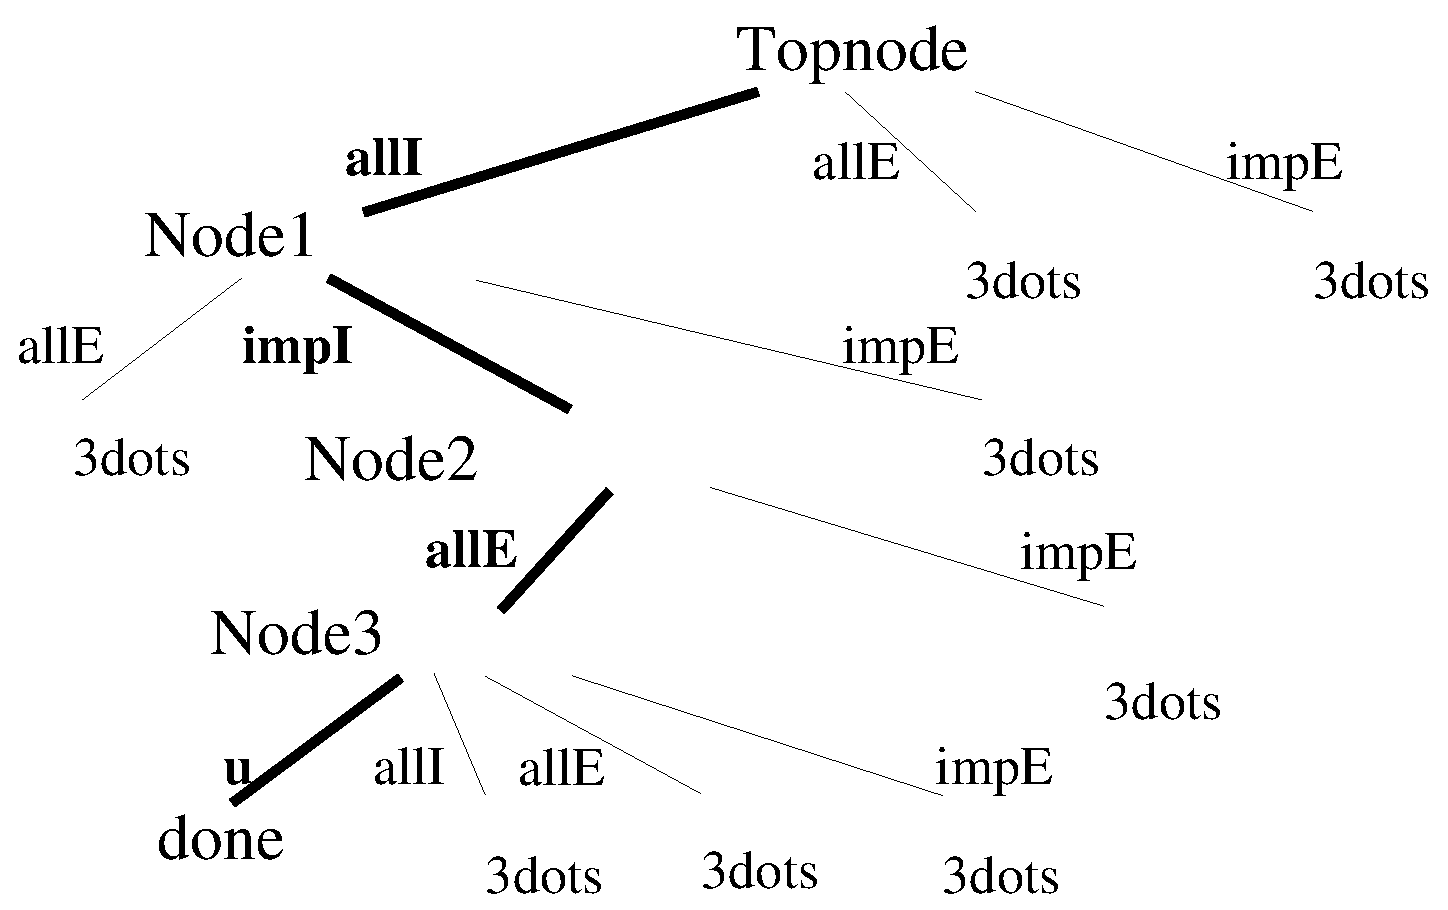
\includegraphics[scale=0.35]{pftree1.eps} 
\end{center}
\end{small}
    \caption{Proof search tree\label{fig:loop3}}
\end{figure}
%\begin{figure}
%\fighead
%\epsfig{file=prooftree1.ps,width=2.7in}
%\caption{\label{prooftree1} Proof Tree for 
%$\top\impl((\top\impl\perp)\impl\perp)$}
%\figfoot
%\end{figure}
      
The top node states the conjecture we are trying to prove. 
Each node is labeled with a goal statement we are trying to prove and
each child node is the result of applying a clause from the program or
from the dynamic clauses. We keep track of which clause has been used
to derive the statement in the child node, by labeling the edge with
the corresponding clause name. The heads of three clauses will unify
with the current goal, namely {\tt allI}, {\tt allE} and {\tt
  impE}. We pick the first of these applicable clauses ({\tt
  allI}). This means we need to solve $\Pi a. \pfLF ( \impLF
(\forallLF \lambda y. P\; y)\; (P a))$. After introducing a new
parameter $a$ applying the {\sf{Universal}} step in out search
procedure, we yield the subgoal $\vd \pfLF ( \impLF (\forallLF \lambda
y. P\; y)\; (P a))$. To prove this subgoal will again inspect our
clauses. Three of them will be applicable, namely {\tt allE}, {\tt
  impI}, and {\tt impE}. This time we will pick the second clause {\tt
  impI}. Hence we will introduce the dynamic assumption {\tt{u}}$ :
\pfLF (\forallLF \lambda y. P\; y)$ and show $\pfLF (P\; y)$ using the
dynamic assumption {\tt{u}}. In the third step, 
again two clauses are applicable,  {\tt allE}, and {\tt
  impE}. Using the first one, {\tt allE}, we need to show that we can
prove $\pfLF (\forallLF \lambda y. P\; y)$. There are four
possible clauses whose clause head will unify: the dynamic clause
{\tt u} and the three program clauses {\tt alli}, {\tt alle}, and {\tt
  impe}. Using the dynamic assumption {\tt u}, we can finish the
proof. Using the labels at the edges we can reconstruct a proof term
for the given query. Twelf's higher-order logic programming engine
will generate the following proof term in explicit form:

% \hspace{-1.25cm}
% \begin{minipage}[h]{6cm}
\begin{code}
(alli {\mygray{($\lambda\!\!$ x. ((forall $\lambda\!\!$ y. P y) imp P x))}}
   $\lambda\!\!$ a. (impi {\mygray{(forall $\lambda\!\!$ y.P y) (P a)}}
           $\lambda\!\!$ u. (alle {\mygray{($\lambda\!\!$ y.P y)}} a u)))).
\end{code}
% \end{minipage}

The final proof term not only tracks the rules which have been used in
every step of the proof, but also tracks the instantiations for the logic
variables in each steps. In the proof term above we show the
instantiations in gray, to denote that they are implicit arguments,
which will be generate during proof search.


% From an operational view point, the search can be described as
% follows: 

%\begin{table}[htbp]
%\fighead
%\begin{small}
%Solve Goal $\Gamma \vd M : G$:
%\begin{enumerate}
%\item $\Gamma \vd (c \cdot S) : G$ \\
%    \mbox{Given an atomic goal $G$ and clauses $\Gamma$:}\hfill\\
%     Focus on a clauses $c : A$ from $\Gamma$ to establish a proof $S$ for $G$.

%\item $\Gamma \vd \lambda u.M : G_1 \arrow G_2$ if $\Gamma, u\oftp G_1
%  \vd M : G_2$ \\
%Augment the clauses in $\Gamma$ with the dynamic assumption $u : G_1$ and
%establish a proof $M$for the goal $G_2$ from the extended  program $\Gamma, u \oftp G_1$.
%\item $\Gamma \vd \lambda a.M : \Pi x. G$ if $\Gamma \vd M : [a/x]G$ where $a$ is a new parameter\\
%Given a universally quantified goal $\Pi x. G$, we
%generate a new parameter $c$, and establish a proof $M$ for $[c/x]G$ in the
% program context $\Gamma$.
%\end{enumerate}
%\end{small}
%\figfoot 
%\caption{Solve goal $G$ from clauses in $\Gamma$}
%\label{tab:solve}
%\end{table}

%Once the goal is atomic, we need to select a clause from the
%program context $\Gamma$ to establish a proof for $G$. In a logic
%program interpreter, we consider all the clauses in $\Gamma$ in order. 
%First, we will consider the dynamic assumptions, and then we will try
%the static program clauses one after the other. 
%Let us assume, we picked a clause $A$ from the program context
%$\Gamma$ and we now need to establish a proof for $G$.

%\begin{table}[h]
%\fighead
%\begin{small}
%Focus on clause $ c : A$ to solve atomic goal $P$.
%\begin{enumerate}
%\item $\Gamma > P' \vd \nil : P$ \\
% Given the atomic clause $P'$ with name $n$, we establish a proof for the
%  atomic goal $P$, by checking  $P' = P$. If yes then
%  succeed. Otherwise fail and backtrack.  
%\item $\Gamma > n : G_2 \arrow G_1 \vd (M ; S) : P$ 
%      if $\Gamma > G_1 \vd S : P$ and  $\Gamma \vd M : G_2$ \\
%  Given the clause $G_2 \arrow G_1$ with name $n$, we establish a
%  proof of the atomic goal $P$, by trying to use the clause $G_1$ to
%  establish a proof $M$ for $P$. If it succeeds, we establish a proof
%  $S$ for the goal $G_2$. If it fails,  backtrack. 
%\item $\Gamma > n : \Pi x\oftp A_1. A_2 \vd S : P$ if $\Gamma > n :
%  [T/x]A_2 \vd (T ; S) : P$\\
%  Given the clause $\Pi x\oftp A_1. A_2$ with name $n$, we
%  establish a proof $(T ; S)$for the atomic goal $P$ by instantiating
%  $x$ with a term $T$, and use the clause $[T/x]A_2$
%  to establish a proof $S$ for the atomic goal $P$. 
%\end{enumerate}
%\end{small}
%\figfoot
%  \caption{Focus on clause $c:A$ to solve atomic goal $P$}
%  \label{tab:foc}
%\end{table}

 Our goal is to reduce the proof evidence to the
non-deterministic choices we have made during the proof to produce
small proof witnesses. In the previous example, it would suffice to
know that in the first step, three possible rules apply, namely {\tt
  alli}, {\tt alle}, and {\tt impe} and we want to follow the first
possibility. In the second step, again three possible rules apply,
namely {\tt alle}, {\tt   impi}, and {\tt impe}, and we want to follow
the second possibility. In the final step, we have four potential
candidates, the dynamic assumption {\tt u: (forall $\lambda\!\!$y P
  y)}, and the rules {\tt allI}, {\tt allE}, and {\tt impE}.
 Hence it would suffice to store only a list of the choices made in
 the proof. In this example, the choices can be characterized by the
 following sequence: $1/3$, $2/3$, $1/2$, $1/4$, keeping in mind that
 dynamic assumptions are tried first by proof search procedures. This
 sequence will constitute our compact proof witness and is all that
 needs to be generated and sent to the verifier. 
      
\section{Oracle-based proof search}
\label{sec:oracles}

In this section, we describe the oracle-based proof generation and
checking. To generate oracles we can follow two ways. First, we will
modify the logic-programming proof search procedure available to generate
a bit-string during proof search directly. As in general logic
programming's depth-first search is incomplete, this may not work
general, although it can be often done with more sophisticated theorem
proving  technology. In certifying code systems however the safety
proof (=proof term) is usually generated by a certifying compiler, and
we merely aim at compressing the safety proof into a bit-string. In
the latter case, we pass into the described search procedure, the
program clauses $\Gamma$, the goal $G$ and the proof term $M$. This
way, we can eliminate all non-determinism from the previous search procedure.

\subsection{Proof compression}

In this section, we will describe the modifications needed to generate
a compact proof witness in form of a bit-string using the verifier's
proof search procedure from the previous section. We assume that we
already have the full proof term and we are merely interested in
compressing the proof term to a small witness in form of a bit-string.
The bit-string encodes the non-deterministic choice within the proof, namely picking
the right clause $c:A$ from the program context $\Gamma$ to establish a
proof $S$ for $P$, once the goal $P$ is atomic, by unifying the head
of $A$ with the atomic goal $P$. Potentially, there is more than one
clause whose head unifies with $P$, and hence a proof search procedure
would need to try all the possible choices in order. The proof witness
just needs to keep track of what possibility was successful.

It is also worth pointing out that in the higher-order setting the
choice of unification algorithm is crucial since not all unification
algorithms are deterministic. Higher-order unification based on Huet's
algorithm \cite{Huet75} for example is highly non-deterministic. On the
other hand higher-order pattern unification \cite{Miller91jlc} is
decidable and deterministic for higher-order patterns. Although it is too restrictive to
concentrate solely on higher-order patterns statically, most of the
non-patterns encountered (for example $(A\;T)$), will become patterns
during execution. Twelf uses higher-order pattern unification together
with constraints \cite{Pfenning91lf}, hence no non-determinism arises
in unification and no additional choices need to be stored in the proof
witness\footnote{Susmit: please check this with Frank}. 

This leads to an efficient encoding of the non-deterministic
choices. If we have $k$ possibilities, we need $\lceil\log_2 k\rceil$
bits. Since we know that the path through the proof tree always has to
lead to a proof, if there is only one choice applying, this formula
correctly says that we do not need to emit an advice.  The verifier
knows how many choices apply, so it can calculate the number of bits
to pick off the oracle. This means that we do not need an explicit
separator between the choices, although we include them here for
better readability. The witness corresponding to the non-deterministic
choices in the previous example is: {\tt 100010101000}.

For the idea to work, proof compression and witness checking
have to perform essentially the same overall proof search. Moreover,
the order in which different choices are considered must be the same.
The only difference is that during witness generation we would explore
possible multiple fruitless paths until settling on the right one,
while in witness checking we know by inspecting the advice encoded in
the bit-string which choice to consider.

We modify the proof search steps presented early such that we pass in
the proof term together with the goal and output a proof witness in
form of a bit-string. Instead of building up a proof term recursively
in the {\sf{Select}}, {\sf{Augment}} and {\sf{Universal}} step, we
only generate the proof witness in the modified {\sf{Select}} step. 
Note that the {\sf{Select}} step is deterministic as the proof term
tells us what choice was successful. It should be intuitively clear
that, we do not necessarily have to pass in the full proof term, but
could directly produce a proof witness in form of a bit-string, if our
proof search is powerful enough that it will eventually find a proof.

\begin{table}[h]
\fighead
\begin{center}
\begin{small}
% \noindent \mbox{{\bf{Solve Goal $\Gamma \vd M: G$:}}\hfill}% \\[-2.5em]
\begin{description}
\item[Select] $\Gamma \vd c_i \cdot S: G \Rightarrow
  \underset{1 \ldots (i-1)}{\underbrace{0\ldots 0}}1\underset{(i+1) \ldots k}{\underbrace{0\ldots 0}}W $ \\
    \mbox{Given an atomic goal $G$ and clauses $\Gamma$:}\hfill\\
    Let $k$ be the number of clauses whose head unifies with the
    current goal $G$ and $c_i : A_i$ be the clause which leads to a
    proof $c_i\cdot S$ of $G$ from $\Gamma$.\\
    Focus on clauses $c_i : A_i$ from $\Gamma$ to compress a proof
     $c\cdot S$ for $G$ to $W$.

\item[Augment] $\Gamma \vd   \lambda u. M : G_1 \arrow G_2 \Rightarrow
  W$ if $\Gamma,
  u\oftp G_1 \vd G_2 \Rightarrow M$ \\
Augment the clauses in $\Gamma$ with the dynamic assumption $u : G_1$ and
compress a proof $M$ for the goal $G_2$ from the extended program
$\Gamma, u \oftp G_1$ to obtain the witness $W$. 
\item[Universal] $\Gamma \vd  \lambda x. M : \Pi x. G \Rightarrow W$ if $\Gamma \vd
  [a/x]M: [a/x]G\Rightarrow W$ where $a$ is a new parameter\\
Given a universally quantified goal $\Pi x. G$, we generate a new
parameter $a$, and compress a proof $[a/x]M$  for $[a/x]G$ in the
program context $\Gamma$ to $W$.
\end{description}
%   \caption{Solve goal $G$ from clauses in $\Gamma$}
\end{small}    
\end{center}
\figfoot
\caption{\label{fig:pwgen}Proof Compression}
\end{table}


%The oracle-string encodes one type of possible choices, but as we
%briefly mentioned earlier, unification in the higher-order setting is
%undecidable in general. In Twelf, we use a higher-order pattern
%unification algorithm together with constraints. Higher-order pattern
%unification is in fact decidable. Although it is too restrictive to
%concentrate solely on higher-order patterns statically, 
%most of the non-patterns encountered (for example $(A\;T)$), will be a
%pattern during execution. Since we assume that we already found a proof $M$
%for a goal $G$ without any left-over unification constraints, 
%all the unification problems solved during execution were
%decidable. It is worth pointing out that our proposal differs here
%from the proposal of Necula and Rahul, who propose to encode the
%non-deterministic choice of Huet's unification algorithm, which does
%not distinguish between higher-order patterns and non-patterns. 

\subsection{Checking small proof witnesses}
In this section, we modify the previous search procedure, in such a
way that it is not parameterized by the proof term $M$, but rather by
the compact proof witness $W$ encoded as a bit-string. Therefore we
have : Solve Goal $\Gamma \vd W : G$, where $W$ is a compact proof witness.  

\begin{table}[h]
\fighead
\begin{center}
\begin{small}
% \noindent \mbox{{\bf{Solve Goal $\Gamma \vd M: G$:}}\hfill}% \\[-2.5em]
\begin{description}
\item[Select] $\Gamma \vd \underset{1 \ldots
    (i-1)}{\underbrace{0\ldots 0}}1\underset{(i+1) \ldots
    k}{\underbrace{0\ldots 0}}W : G $ \\
    \mbox{Given an atomic goal $G$ and clauses $\Gamma$:}\hfill\\
    Let $k$ be the number of clauses whose head unifies with the
    current goal $G$, then inspect the first $k$ bits, and
    find the $i$-th bit which is one.\\  
    Focus on clauses $c_i : A_i$ from $\Gamma$ to establish a proof
    for the atomic goal $G$ from $\Gamma$ using remaining proof witness $W$.
\end{description}
%   \caption{Solve goal $G$ from clauses in $\Gamma$}
\end{small}    
\end{center}
\figfoot
\caption{\label{fig:pwgen} Proof Reconstruction}
\end{table}

In {\sf{Select}} step, we first generate the $k$ possible candidates whose
head will unify with the current goal $G$. If $k$ is greater than 1, we
will take off $k$ bits from the witness. If a bit $1$ occurs at
position $ip$ of these $k$ bits, we will pick the $i$-th candidate.

To check that proof witnesses in fact constitute a valid proof for a
given proposition, we re-run the prover guided with the advice encoded
in the bit-string. The witness checker is then in fact a deterministic
search procedure. No backtracking is necessary, since all the
non-deterministic choices are resolved.  By taking the appropriate
branches (and performing the needed unification), the user can be convinced that such a
proof exists. This can lead to savings of time and memory.
This however requires the code consumer to trust the witness
checker -- which includes trusting higher-order pattern
unification. For a paranoid consumer this may be unacceptable since
the witness checker may use optimizations such as caching subproofs
and indexing, which can be quite complicated. In this case, it is
possible to also output a full proof term as a result of the guided
proof search. This amounts to decompressing the proof witness $W$to an
explicit proof term $M$ and use a different trusted type-checker to
verify the expanded proof witness. 

\section{Optimizations: Higher-order Term Indexing}

A proof search procedure must have a way of retrieving all clauses of
the logic program which may satisfy the current goal, since such a
method will dictate how many choices we are returned at any step, and
hence is critical in understanding the oracle. Most first-order logic
programming interpreter use term indexing strategies to efficiently
retrieve all clauses whose head unifies with the current goal.

In the higher-order setting, indexing strategies for higher-order
terms are difficult, since in general retrieval and often also
insertion operations rely on computing the most general unifier or the
most specific generalization. However, in the higher-order case,
unification is in general undecidable and the mgu does not necessarily
exist. The same holds for computing the most specific generalization
of two terms. As discovered by Miller \cite{Miller91iclp}, there exists a decidable
fragment, called higher-order patterns. For this fragment, unification
and computing the most specific generalization is decidable even in
rich type theories with dependent types and polymorphism as shown by
Pfenning \cite{Pfenning91lics}.  However, these algorithms, which must
compute bound variable dependencies, may not be efficient in practice
\cite{PientkaPfenning:CADE03}.  

For the purpose of this paper, we will adopt higher-order substitution
trees as described in \cite{Pientka:ICLP03}. Substitution tree
indexing has been successfully used in a first-order setting \cite{Graf+Book95} and
allows the sharing of common sub-expressions via substitutions. This
is unlike other non-adaptive term indexing, which only allow sharing
of common term prefixes. To extend substitution tree indexing to the
higher-order setting, we will concentrate on the fragment of linear
higher-order patterns, where all existential variables must occur only
once and are applied to all distinct bound variables. Linear
higher-order patterns refine the notion of higher-order patterns
\cite{Miller91iclp}, where all existential variables must be applied
to a some distinct bound variables. 

 In \cite{Pientka:ICLP03,Pientka03phd}, we give a formal 
description for computing the most specific generalization of two
linear higher-order patterns, for inserting terms in the index and for
retrieving a set of terms from the index s.t. the query is an instance
of the term in the index, and show correctness. This can be extended
to unifiability. The construction of a substitution tree in the higher-order setting
follows the overall algorithm described in
\cite{Ramakrishnan01:indexing}. The crucial part to adapt substitution
trees to the higher-order setting is the notion of linear higher-order
patterns.

For this setup to work cleanly in the higher-order
setting, it is crucial that we distinguish between existential
variables in $\Delta$ and bound variables and assumptions in
$\Gamma$. Moreover, it is essential that existential variables allow
in place up-date. In particular, we will rely on the notion of
existential variables which are ``fully applied'', i.e. they may
depend on all the bound variables they occur in.

A higher-order substitution tree is a tree whose
nodes are substitutions. It is crucial that any internal variable $i$
is treated as an existential variable which is applied to all the
variable in whose scope it occurs in. By composing the substitutions along a path,
we will obtain a term. To illustrate, consider the following
set of clauses describing part of a conversion of formulas into prenex
normalform. 

\begin{small}
\[
\begin{array}{l}
\eqLF :\;  \propLF \rightarrow \propLF \rightarrow \typeLF.\\[1em]
%
\eqilLF: \eqLF (\impLF (\existsLF \lambda x. A\; x)\; B)\quad (\forallLF \lambda x. (\impLF (A\; x)\; B)).\\
\eqirLF: \eqLF (\impLF A\; (\forallLF \lambda x. B\;x)) \quad (\forallLF \lambda x. (\impLF A \; (B\; x))).\\
\eqalLF: \eqLF (\andLF (\forallLF \lambda x. A \;x) \; B)\quad (\forallLF \lambda x. (\andLF (A\; x)\; B)).\\
\eqarLF: \eqLF (\andLF A \; (\forallLF \lambda x. B\; x)) \quad (\forallLF \lambda x. (\andLF A \; (B\;x))).\\
\end{array}
\]
\end{small}

We see that the four given clauses share a lot of structure. For
example clause $\eqilLF$ and $\eqirLF$ ``almost'' agree on the second
argument. Similarly the clauses $\eqalLF$ and $\eqarLF$. To insert
these four clauses into a substitution tree, we need to first
translate them into linear higher-order patterns. Although all the
terms in these clauses fall into the pattern fragment, since all the
existential variables are applied to distinct variables, not all of
them are applied to {\em{all}} distinct bound variables. For example, 
\[
\eqLF (\impLF (\existsLF \lambda x. A\; x)\; B)\quad (\forallLF
\lambda x. (\impLF (A\; x)\; B)
\]

the existential variable $B$ does not depend on the bound variable
$x$, in $(\forallLF \lambda x. (\impLF (A\; x)\; B)$. Hence, $B$ is
not a linear higher-order pattern, since it it not applied to all
bound variables in whose scope it occurs. In addition, the existential
variable $A$ occurs twice. Before inserting the clause heads into a
substitution tree, we first linearize them, eliminating any duplicate
occurrences of existential variables, and replacing any existential
variable which is not fully applied with one which is. The program after
linearization is shown next:

\begin{small}
\[
\begin{array}{ll}
% \eqLF: \quad \propLF \rightarrow \propLF \rightarrow \typeLF.\\[1em]
%
\eqilLF: \eqLF (\impLF (\existsLF \lambda x. A\; x)\; B)\;
                 (\forallLF \lambda x. (\impLF (A'\; x)\; (B'\;x))). \\
\hspace{1cm}\forall x. (A'\; x) \unif (A \; x) {\textsf{ and } } B'\;x   \unif B\\[0.5em]
\eqirLF: \eqLF (\impLF A\; (\forallLF \lambda x. B\;x))\quad
                 (\forallLF \lambda x. (\impLF (A'\;x) \; (B'\; x))).\\
\hspace{1cm} \forall x. (A'\; x) \unif A  {\textsf{ and }} B'\;x   \unif (B\;x)\\[0.5em]
\eqalLF: \eqLF (\andLF (\forallLF \lambda x. A \;x) \; B)\quad
                 (\forallLF \lambda x. \andLF (A'\; x) \; (B'\;x)).\\
\hspace{1cm} \forall x. (A'\; x) \unif (A \; x) {\textsf{ and }} B'\;x   \unif B\\[0.5em]
\eqarLF: \eqLF (\andLF A \; (\forallLF \lambda x. B\; x)) \quad
                 (\forallLF \lambda x. \andLF (A'\;x) \; (B' x)).\\
\hspace{1cm} \forall x. (A'\; x) \unif A  {\textsf{ and }} B'\;x   \unif (B\;x)\\[0.5em]
\end{array}
\]
\end{small}

Now even more sharing becomes apparent. For example, the clauses
$\eqilLF$ and $\eqirLF$ agree upon the last argument. Similarly, the
clauses $\eqalLF$ and $\eqarLF$. We now compute the most specific
generalization between these clauses, and can build up a substitution
tree. The algorithm for computing the most specific generalization is
given in \cite{Pientka03phd,Pientka:ICLP03}.

\begin{note}
  Should be repeat it here? -- Or at least point out the use of modal
  variables which are lowered?
\end{note}

\begin{figure*}[htbp]
  \begin{center}
    \begin{small}
% nodesep=1pt,
\pstree[nodesep=0.5pt,levelsep=8ex]{%
\TR{$\eqLF\quad i_2 \quad (\forallLF \lambda x. i_1\;x)$} }{%
  \pstree{\TR{\begin{tabular}{r}
              $\lambda x.(\andLF (A'\;x)\; (B'\;x))/i_1$\\
              $(\andLF (i_3\;x)\; (i_4 \;x))/i_2$\\
            \end{tabular}
          }
        }{%
          \pstree{\TR{\begin{tabular}{r}
                $\lambda y.(\forallLF \lambda x. A\;x)/i_3$,\\
                ${\tt \lambda y.B/i_4}$
              \end{tabular}
            }}{%
            \pstree{\TR{\begin{tabular}{l}
                  $\forall x. A'\;x\unif A\;x$\\
                  $B'\;x\unif B$
                \end{tabular}
              }}{ $\eqarLF$}
          }
%
          \pstree{\TR{\begin{tabular}{r}
                ${\tt \lambda y.A/i_3},$\\
                $\lambda y.(\forallLF \lambda x. (B\;x))/i_4$
              \end{tabular}
            }
          }{%
            \pstree{\TR{\begin{tabular}{l}
                $\forall x. A'\;x\unif A$\\
                $B'\;x \unif B\;x$
              \end{tabular}
            }
            }{ $\eqalLF$}
          }
        }
%%%%% second child
          \pstree{\TR{\begin{tabular}{r}
                     $\lambda x.(\impLF (A'\;x)\; (B'\;x))/i_1$\\
                     $(\impLF i_3\;x\; i_4\;x)/i_2$\\
                   \end{tabular}
                 }}{
                 \pstree{\TR{\begin{tabular}{r}
                       $\lambda y.\forallLF \lambda x. A\;x/i_3$,\\
                       ${\tt \lambda y.B/i_4}$
                       \end{tabular}
                     } }{%
                     \pstree{\TR{\begin{tabular}{l}
                           $\forall x. A'\;x\unif A\;x$\\
                           $\forall x. B'\;x\unif B$
                         \end{tabular}}
                     }{$\eqirLF$}
                   }
                  \pstree{\TR{\begin{tabular}{r}
                        ${\tt \lambda y.A/i_3},$\\
                        $\lambda y.(\forallLF \lambda x.B\;x)/i_4$
                      \end{tabular}}}{
                    \pstree{\TR{\begin{tabular}{l}
                          $\forall x. A'\;x \unif A$\\
                          $\forall x. B'\;x \unif B\;x$
                        \end{tabular}}
                    }{$\eqilLF$}
                  }
                }
              }     
    \end{small}
  \end{center}
  \caption{Substitution tree}
  \label{fig:substree}
\end{figure*}

% \end{small}

By composing the substitutions along a path,
we will obtain a clause head. By composing the substitutions in the
left-most branch, we obtain the clause head $\eqalLF$.  
In contrast to other indexing techniques such as discrimination tries,
substitution trees  allows the sharing of common sub-expressions
instead of common term prefixes. As we can see in this example, this
is especially useful in this example, since the most sharing is done
in the second argument. 

We have chosen to index only the static set of program clauses. In
theory, it is possible to use substitution tree indexing for dynamic
clauses generated during proof search.  However, it is not clear how
useful this will be, since the process of creating the tree itself is
time-consuming. It is also noted by Necula and Rahul \cite{Necula+01:oracle} that
indexing dynamic assumptions imposes a performance penalty. It is
useful to pre-process the program, but the payoff with dynamic clauses
is unclear. For dynamic clauses, we use only simple indexing on the
type family of type.

\begin{note}
  \begin{itemize}
  \item Should we talk about lowered terms and modal variables
  \item Should be give an algorithm for computing the most specific
    generalization? (it is given in ICLP'03)
  \end{itemize}
\end{note}


\section{Caching results}
\label{sec:tabling}
Since large proofs often have identical subproofs,  there is a
lot of opportunity for sharing subproofs. The problem is particularly
acute in machine-generated proofs for certifying machine-code which
tend to have repeated proofs of simple facts. This problem has been
already pointed out by Necula and Lee in \cite{NeculaLee+97:resource}

 \begin{tabular}[h]{l}
``...it is very common for the proofs to have  \\
repeated sub-proofs that should be hoisted out and \\
proved only once ...'' \cite{NeculaLee+97:resource}\\ $\;$
 \end{tabular}


In the context of oracle-based proof checking, this leads to two
problems.  First, the oracles become larger in size than
necessary. This means that what has to be transmitted to the verifier
is large in size. Secondly, the performance of witness checker may
degrade, since it spends its time uselessly proving the same fact over
and over again. 

Ideally we would like to cache intermediate results and re-use them
later. Up to now, this has been difficult since we need to efficiently
store and retrieve intermediate goals. We adapt and build upon recent
work \cite{Pientka03phd} on memoizing intermediate goals during
execution as part of the tabled higher-order logic programming and
adapt it for witness generation and witness checking. 

When we generate compressed witnesses for a goal $G$ from explicit
proof terms, we store intermediate goals together with their
compressed witness in a table, and re-use the result later on. 
We will modify the {\sf{Select}} step in our previous search procedure
to allow for tabling as follows.

\begin{table}[h]
\fighead
\begin{center}
\begin{small}
% \noindent \mbox{{\bf{Solve Goal $\Gamma \vd M: G$:}}\hfill}% \\[-2.5em]
\begin{description}
\item[Select-Cache] $\Gamma \vd c_i \cdot S: G \Rightarrow
  \underset{1 \ldots (i-1)}{\underbrace{0\ldots 0}}1\underset{(i+1) \ldots k}{\underbrace{0\ldots 0}}W $ \\
    \mbox{Given an atomic goal $G$ and clauses $\Gamma$:}\hfill\\
    Let $k$ be the number of clauses whose head unifies with the
    current goal $G$ and $c_i : A_i$ be the clause which leads to a
    proof $c_i\cdot S$ of $G$ from $\Gamma$.\\
    {\em{if CallCheck($\Gamma \vd G$, \cal{T}) \\
         then return a pointer to the answer list and\\
        \hspace{0.5cm}reuse the answers\\
      otherwise}} \\
\hspace{0.5cm}Focus on clauses $c_i : A_i$ from $\Gamma$ to compress
\\
\hspace{0.5cm}a proof $c\cdot S$ for $G$ to $W$.\\
     \hspace{0.5cm}{\em{Add $\Gamma \vd G$ together with the proof
         witness $W$\\
\hspace{0.5cm}to the table $\cal{T}$}}
\end{description}
%   \caption{Solve goal $G$ from clauses in $\Gamma$}
\end{small}    
\end{center}
\figfoot
\caption{\label{fig:pwgen} Proof Compression with Caching}
\end{table}

{\em{CallCheck($\Gamma \vd G, \cal{T}$)}} checks whether a variant of
the current subgoal exists or if the current subgoal is an instance of
a previous entry. If there exists a table entry $\Gamma' \vd P'$
s.t. $\Gamma \vd P$ is a variant (or instance) of the already existing
entry $\Gamma' \vd P'$. A naive implementation can result in
repeatedly rescanning terms and thereby degrading performance
considerably. Moreover, a naive implementation may not be space
efficient, if it does not take advantage of sharing common structure
and common operations. We use higher-order substitution tree indexing
to store intermediate goals $G$ together with their dynamic
assumptions $\Gamma$ and the corresponding proof witness
$W$. Typically intermediate goal $G$ may contain existential
variables which are realized via references and destructive updates in
an implementation. This achieves that instantiations of existential variables
are immediate. On the other hand instantiations for existential
variables may need to be rolled back upon backtracking, in other words
the state of the existential variables may change during proof search.
Hence when tabling a given subgoal, we must abstract over all the
existential variables and store an abstract version of the
subgoal to avoid the pollution of the table entries.
Hence before adding a subgoal with existential variables, we will
abstract over them and standardize the goal together with its dynamic
assumptions. 

\[
\begin{array}{lclclcl}
\multicolumn{1}{c}{\Delta} & ; & \multicolumn{1}{c}{\Gamma} & \vd &
\multicolumn{1}{c}{G}
& / & \multicolumn{1}{c}{R}\\
 \end{array}
\]

$\Delta$ refers to a context describing existential variables,
$\Gamma$ describes the context for the bound variables  and dynamic
assumptions and $G$ describes the goal we are attempting to prove. 
In addition, we translate every subgoal into a linear higher-order pattern
together with some residual constraints $R$, so we can insert it into a
higher-order substitution tree.

To allow easy comparison of goals $G$ with dynamic assumptions
$\Gamma$ modulo renaming of existential variables and bound variables, we
represent terms internally using explicit substitutions
\cite{Abadi:POPL90} and de Bruijn indices. The basic underlying idea
is to use a nameless representation of variables based on de Bruijn
indices. The main advantage is that equality up to renaming
of bound variables is reduced to syntactic equality checks, if all
objects are in $\beta\eta$-normalform.

Once this subgoal is solved and we inferred a possible instantiation for
the existential variables in $\Delta$, we will add the answer to the
table. The answer is a substitution for the existential variables in
$\Delta$. In general, the
answer substitution may also contain existential variable itself, over
which we must abstract, when adding the answer substitution to the
table\ednote{Give an example? -bp}.

\begin{note}
  Susmit: Are we really first checking if $\Gamma \vd G$ is in the
  table, and then later on we insert it???
  
   Maybe the answer is: In proof compression, we care more about
   obtaining the shortest possible proof witness than the performance
   of compressing proofs. 

  Susmit: Are you only using variant checking or are you also using
  subsumption?

  Susmit: How big is the table? Are we just memoizing *every* possible
  subgoal encountered or are we selectively memoizing?

  Susmit: Are we caching everything or are we caching selectively?
\end{note}

The following important invariants hold about the table

\[
\begin{array}{ll}
\mbox{Table entry} & \Delta ; \Gamma \vd G\\
\mbox{Residual Equ.} & \Delta ; \Gamma \vd R \\
\mbox{Answer substitution} & \Delta' \vd \theta : \Delta
\end{array}
\]

The design supports naturally substitution factoring based on explicit
substitutions\cite{RamakrishnanJLP99}. With substitution factoring the
access cost is proportional to the size of the answer substitution
rather than the size of the answer itself. It guarantees that we only
store the answer substitutions, and create a mechanism of returning
answers to active subgoals that takes time linear in the size of the
answer substitution $s$ rather than the size of the solved query
$[\theta]G$. In other words, substitution factoring ensures that answer
tables contain no information that also exists in their associated
call table. Operationally, this means that the constant symbols in the
subgoal need not be examined again during either answer check/insert
or answer backtracking. For this setup to work
cleanly in the higher-order setting, it is crucial that we distinguish
between existential variables in $\Delta$ and bound variables and
assumptions in $\Gamma$. Moreover, it is essential that existential
variables allow in place up-date.  In the following, we will describe
requirements and challenges we face of memoizing sub-goals in the
higher-order setting. 

\subsection{Optimization: Strengthening and subsumption}

Apply strengthening to detect more identical subproofs (strengthening
based on subordination and on not adding dynamic assumption twice)

The stored solution to a tabled goal is not always the solution we
want to use.  This is because using a particular answer will constrain
the free variables, possibly in ways not helpful to the proof. 

We add the choices from the table to the menu of choices available at
every choice point. Again, both the prover and verifier are following
similar algorithms, so both have identical caches. The number of
choices is also the same in both the prover and verifier. We just need
a convention on how to specify a tabled answer, and we choose the
choices appearing in the table to precede the other choices.

\begin{note}
  Say more about strengthening; is it critical in the proofs about the
  sequent calculus?  
\end{note}
\section{Experimental Results}

We show an extensive experimental evaluation of the generating and
checking proofs using compact proof witnesses.

\begin{note}
This evaluation should show:
\begin{itemize}
\item Time of proof checking vs proof reconstruction using small
  witnesses
\item Size of proof term vs Size of witness 
\item Size of witness without caching vs Size of witnesses with
  caching
\item Size of the cache
\item Time for proof compression using caching vs Time for proof
  compression without caching (is there a performance penalty?)
\item Overhead of using Twelf for proof compression vs using a
  specialized system like Fleet?
\end{itemize}
\end{note}

\subsection{Foundational Proof Carrying Code}
Here we consider the typed assembly language. The type system
guarantees safety.

\subsection{Sequent Calculus as a general Safety Logic}
Here we consider the sequent calculus as a general safety logic.

\subsection{Refinement Types as an advanced type system}
In this section, we consider an advanced type system based on
refinement types for a high-level ML-like language. 


\section{Related Work}
The idea of using oracles which encode the non-deterministic choice in
a logic programming interpreter was first proposed by
\cite{Necula+01:oracle} for a fragment of the logical framework LF,
called LF$_i$. Their main goal was to design a practical method for
the current proof-carrying code applications which would reduce the
size of proofs. To achieve this goal, the compromised at different
ends to suit their needs. First, they concentrate on the 
fragment $LF_i$, which concentrates on 2-level fragment of
LF. To index program clauses, they propose the use of automata-driven
indexing, where any higher-order features are ignored. Their
indexing algorithm will generate a set of potential candidates, which
may include candidates which are unsound. To weed out the unsound
candidates, full higher-order unification based on Huet's algorithm is
called. This is clearly wasteful, since we will traverse higher-order
terms at least twice. Moreover, since they use Huet's unification
algorithm, which is non-deterministic itself, their theoretical
proposal includes encoding the choices made within higher-order
unification. To avoid these higher-order problems in practice, their
realization and their experimental evaluation does not consider 
terms defined via $\lambda$-abstraction. To handle some simple cases
like the {\tt alli} rule in our example, they introduce a hack to deal
with this special case. 

In fact, one can say that  our work continues where Necula and Rahul
left of saying ``more experimental results are needed especially in
the higher-order setting''. Our work extends this approach to full LF
by removing any of these restriction, and incorporating higher-order
term indexing as well as caching intermediate results.

There is also
an important difference in how we generate bit-strings:

\begin{note}
  Susmit: say more about the difference and why ours is better.
\end{note}

The idea of using oracles was also explored in
\cite{Appel:PPDP03}. Their primary concern was to 
achieve a minimal proof checker, in terms of number of lines of
code. Their checker follows the path explored by Necula and Rahul and
ignores higher-order terms. The main difference between the two
approaches is that the proof rules are proven correct
independently thereby minimizing the trusted computing base.
As Necula and Rahul's work, their system is not able to support
higher-order abstract syntax, which means that  
that any variable binding constructs must be
explicitly encoded. Wu {\em et al}\cite{Appel:PPDP03}
encode the explicit substitution calculus \cite{Abadi:POPL90} together
with the necessary proofs about substitutions for their foundational
implementation of LTAL. Although the overhead in this setting is still
manageable, it is not general enough to handle richer safety polices.

 Our work fills this gap by describing a general purpose tool to
 compress proofs to compact witnesses and check proofs for the logical
framework LF. We demonstrate that the restrictions to first-order terms
are unnecessary. 

\section{Conclusion}


\bibliographystyle{plain}
\bibliography{biblio}
\end{document}



